\section{2.4 Разработанные индексы и алгоритмы}

\subsection{2.4.1 Geohash B-tree}
Во время разработки системы тестирования (рисунок 12), было замечено, что алгоритм \textit{перебора} достаточно хорошо работает на задаче «КНН 25\%». Данная задача требует от алгоритма вернуть K ближайших точек, где $K = \frac{N}{4}$, где N - общее кол-во точек массива. 
  \\
\begin{figure}[h]
    \centering
    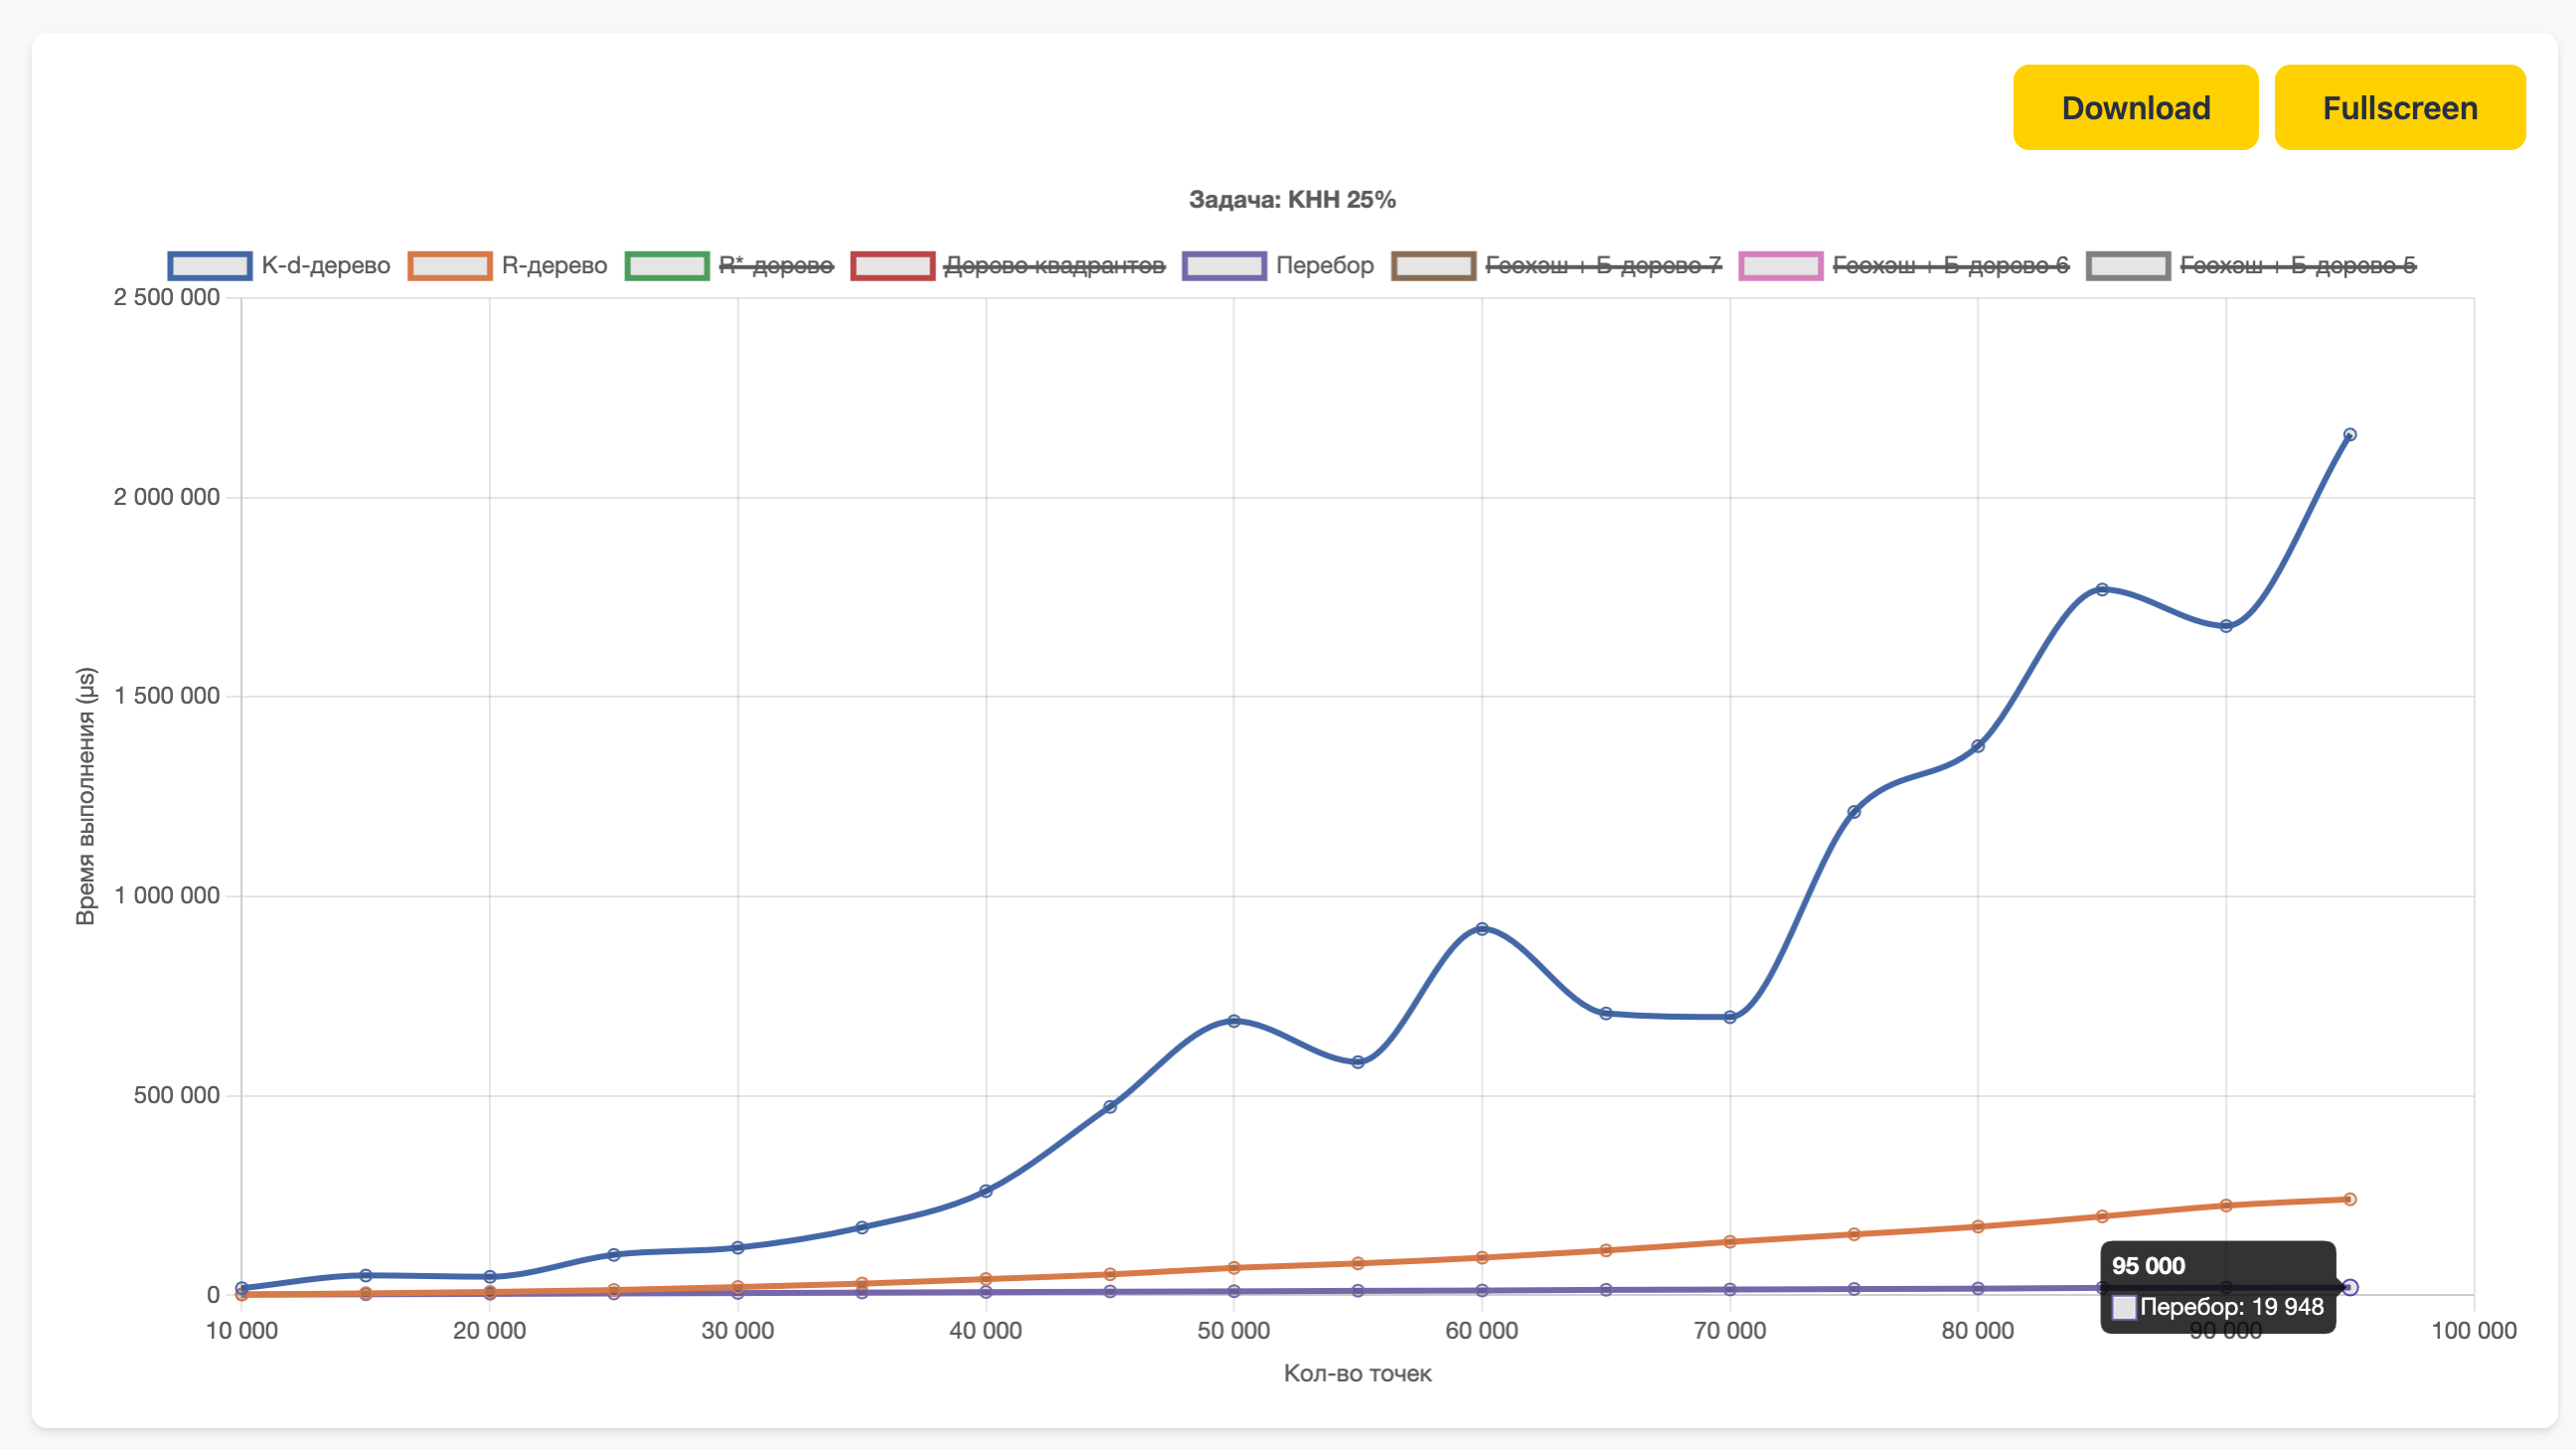
\includegraphics[scale=0.3]{result_knn_bruteforce.png}
    \caption{Результаты тестирования}
\end{figure}
  \\
Иными словами, алгоритм простого перебора показывает хорошие результаты, когда K близко или сравнимо с N ($K \centernot \ll N$), что было взято за основу алгоритма «Geohash B-tree». 

Устройство разработанного «Geohash B-tree» просто, индекс представляет собой B-Tree\cite{comerBTree}, ключами которого являются геохеши в типе данных uint64, а значениями - массив точек, которые находятся в указанном хеше. Размерность является параметром индекса и фиксируется. Для реализации алгоритмов поиска применяется возможность геохеша кластеризовать пространство земли и находить кластеры, в которых уже далее \textit{перебором} производятся операции поиска по KNN или BBox\cite{gulakovStructured}.

Итерации поиска в прямоугольнике (рисунок 13)
\begin{enumerate}
    \item Получить геохеши углов, в примере на рисунке 13 - \textit{5} и \textit{y} (если опускать общий префикс)
    \item Получить все точки, что находятся на гранях прямоугольника (\textit{5}, \textit{h}, \textit{j}, \textit{n} и тд.)
    \item Данные точки требуется также проверить на вхождение в прямоугольник через простой перебор
    \item Все точки, что входят во внутрь (\textit{k}, \textit{s}, \textit{m}, \textit{t}) - проверять не надо, они гарантированно входят в прямоугольник
\end{enumerate}
  \\
\begin{figure}[h]
    \centering
    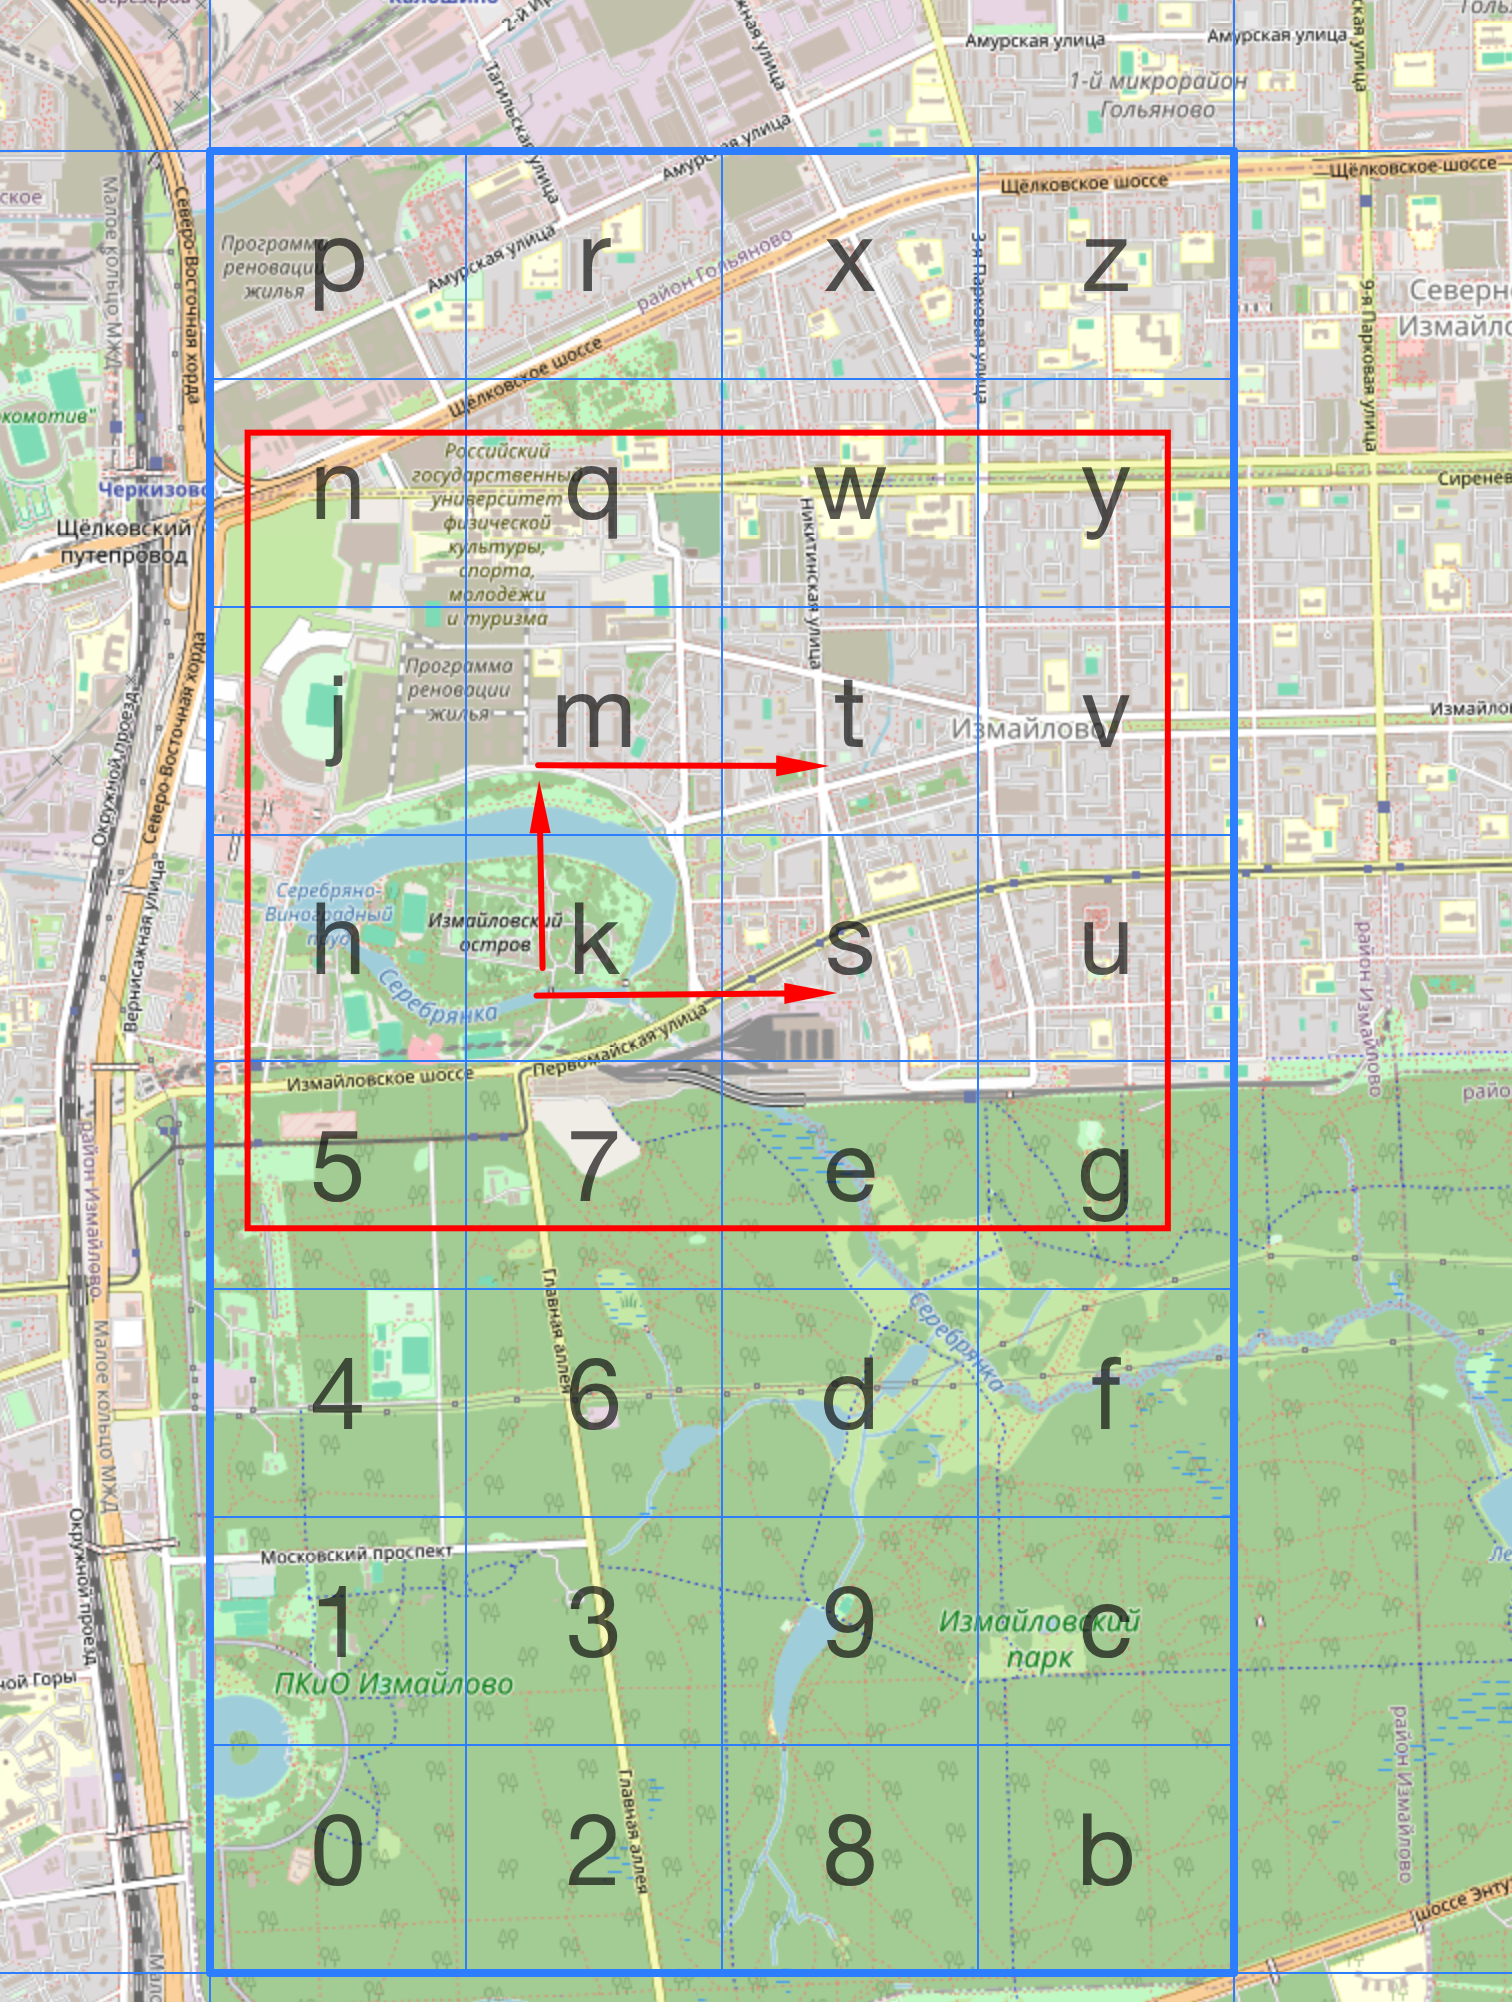
\includegraphics[scale=0.3]{geohash_btree_bbox.png}
    \caption{Алгоритм поиска в прямоугольнике}
\end{figure}
  \\
Итерации поиска ближайшего соседа (рисунок 14)
\begin{enumerate}
    \item Найти геохеш точки P. В примере на рисунке 14 - \textit{ucfv7m}
    \item Получить все точки, в указанном геохеше
    \item По часовой стрелке итерироваться по соседям оригинального геохеша и выгружать точки. (ucfv7m -> ucfv7q -> ucfv7w и тд)
    \item Завершить итерацию, когда кол-во найденных точек будет больше или равно K
    \item Найти наиболее дальшестоящую точку из найденного массива относительно заданной точки P. Пусть расстояние между указанными точками будет R 
    \item Найти все точки в прямоугольнике, с центром в P и сторонами 2R.
    \item Точки в полученном массиве отсортировать по расстоянию и выдать первые K точек
\end{enumerate}
  \\
\begin{figure}[h]
    \centering
    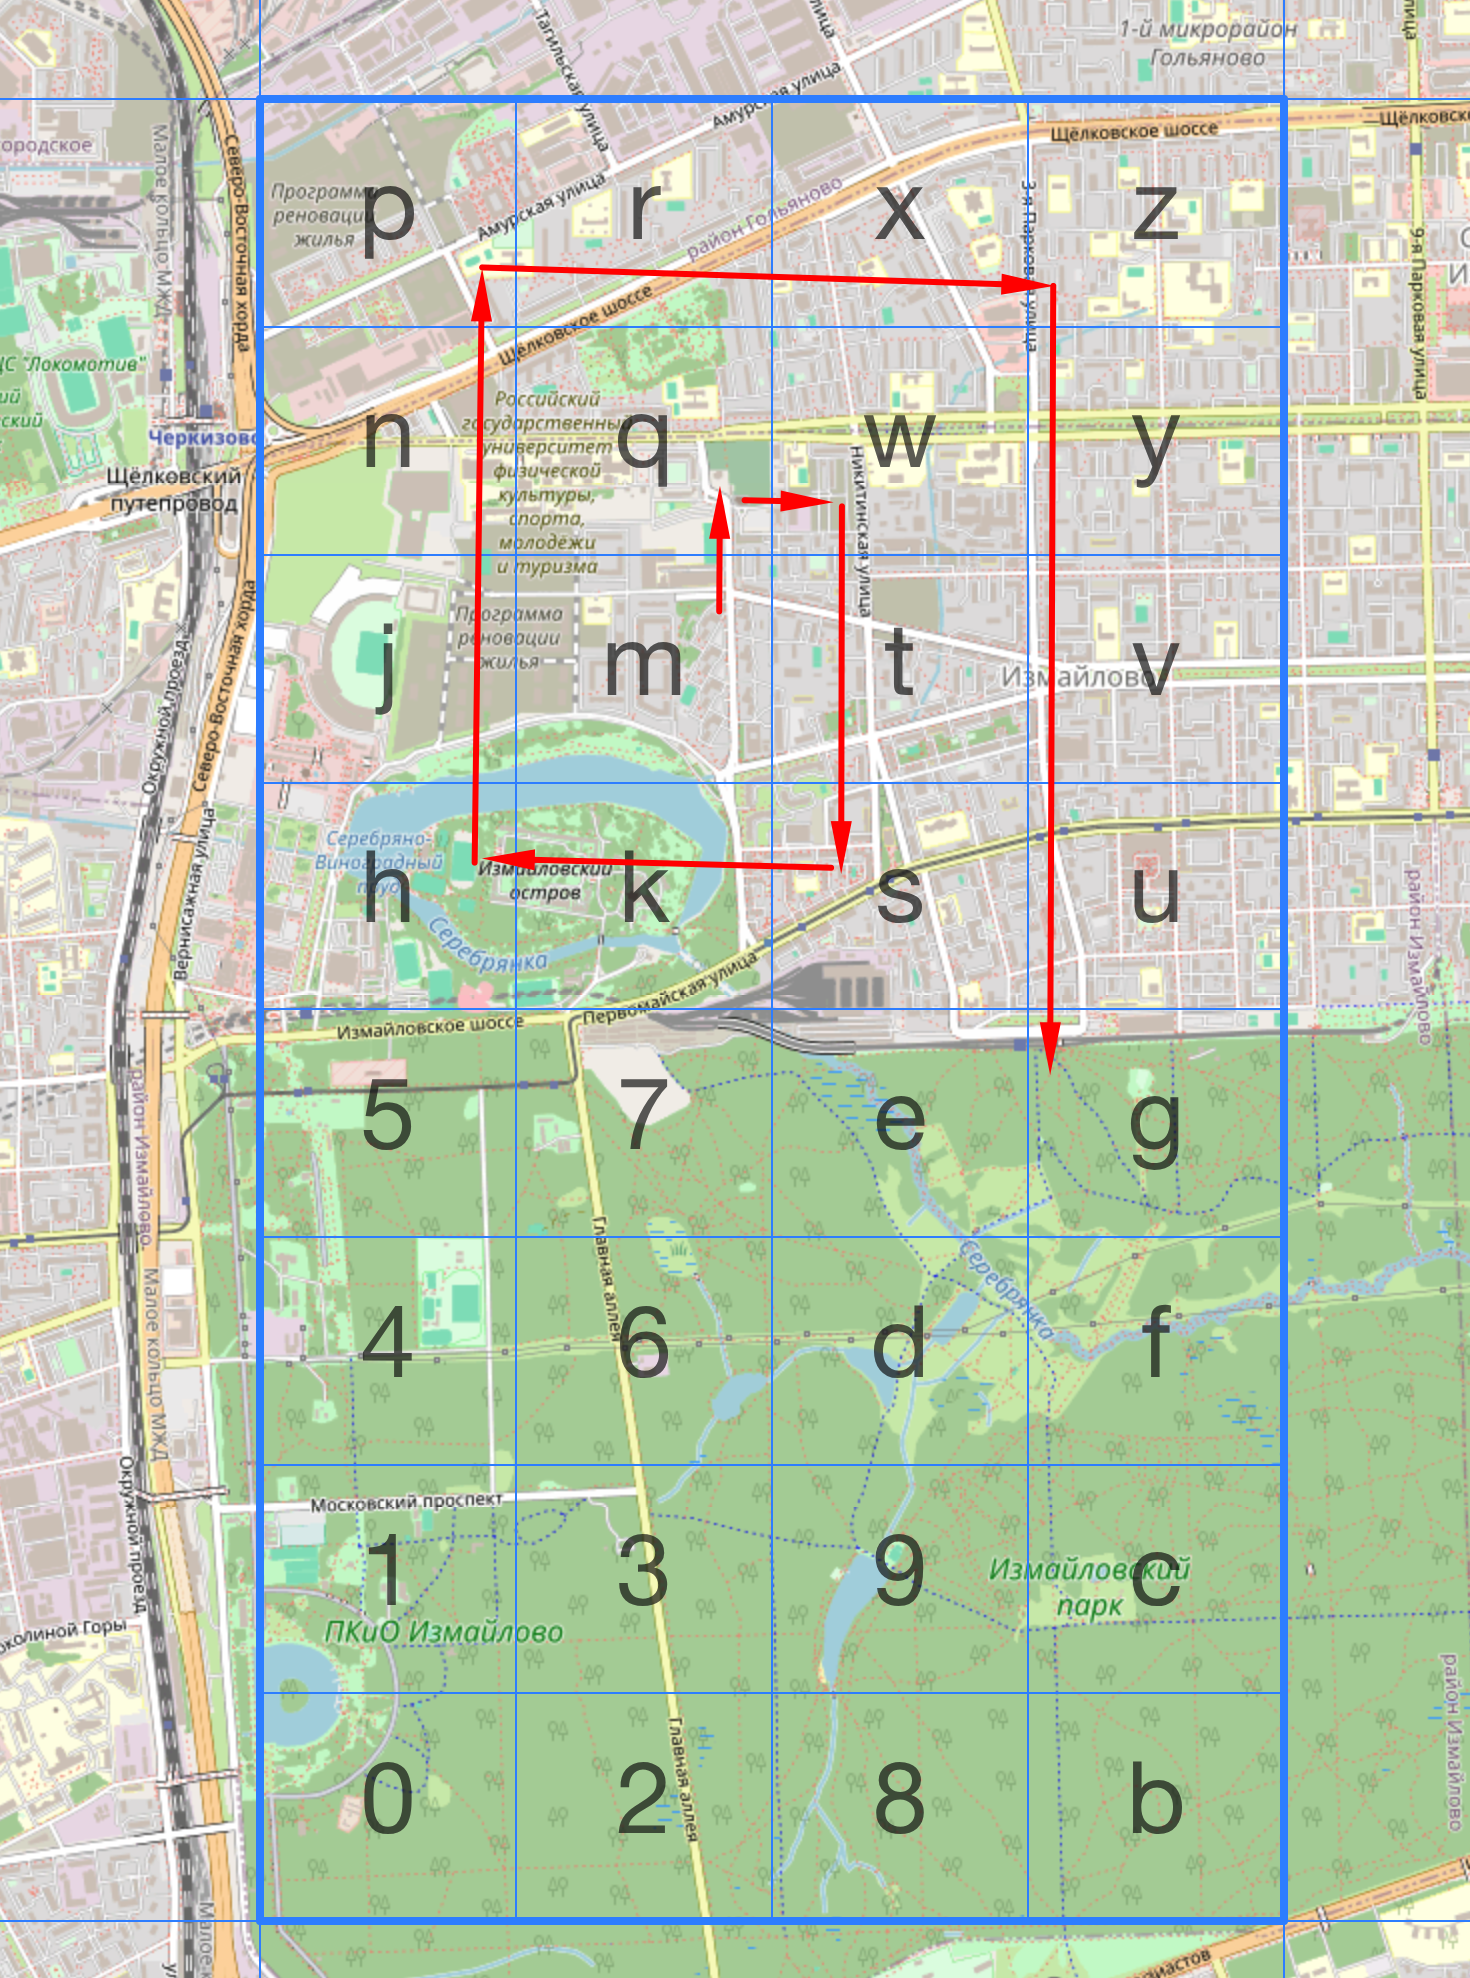
\includegraphics[scale=0.3]{geohash_btree_knn.png}
    \caption{Итеративный проход по соседям}
\end{figure}
  \\
У разработанного алгоритма крайне много преимуществ
\begin{enumerate}
    \item Клиентский. Может быть полностью реализован на стороне клиента, а не СУБД. Если СУБД не поддерживает какие-либо геоиндексы, как например AWS DynamoDB, данный индекс можно использовать для закрытия потребности в геоиндексах. 
    \item Кластерезируемый. В отличие от R-Tree, данный индекс без проблем реализует кластеризацию. Также важно отметить, что B-Tree в данном индексе использует только операции Get и Set, без сравнения и итераций, за счет чего данный индекс можно применять, например, в СУБД Redis, которая нативно поддерживает кластеризацию ключей 
    \item Комбинируемый. В случае необходимости, его можно комбинировать с R-Tree, например, для СУДБ Redis можно хранить в ключах, а в значениях - R-tree через операцию \textit{GEOADD}\cite{redisGeo}
\end{enumerate}
Но также имеется много минусов
\begin{enumerate}
    \item Параметризируемость. На создание индекса требуется выбрать размерность Geohash, она не может быть изменена. Если выбранная размерность будет слишком большой или слишком малой, производительность индекса будет слишком низкой. 
    \item Крайние случаи. Если клиент отправит запрос на задачу KNN, при этом в указанной точке и рядом не будет точек, индекс будет медленно итерироваться по всем ближайшим геохешам.
\end{enumerate}